\documentclass[conference]{IEEEtran}
\IEEEoverridecommandlockouts

\usepackage{cite}
\usepackage{amsmath,amssymb,amsfonts}
\usepackage{algorithmic}
\usepackage{graphicx}
\usepackage{textcomp}
\usepackage{xcolor}
\usepackage{hyperref}
\usepackage{booktabs}
\usepackage{multirow}
\usepackage{adjustbox}
\usepackage{float}

\graphicspath{{figures/}}

\def\BibTeX{{\rm B\kern-.05em{\sc i\kern-.025em b}\kern-.08em
    T\kern-.1667em\lower.7ex\hbox{E}\kern-.125emX}}

\begin{document}

\title{A Calibrated Dynamic Microsimulation Framework for Assessing Retirement Adequacy under Alternative Migration, Wealth, and Statutory Pension Scenarios in Germany (2025--2070)}

\author{
    \IEEEauthorblockN{Cristhian David Caceres Mateus$^{1}$}
    \IEEEauthorblockA{$^{1}$University of Europe for Applied Sciences, Potsdam, Germany}
    \IEEEauthorblockA{e-mail: cristhian.caceres@ue-germany.de}
}

\maketitle

\begin{abstract}
Germany faces dual structural pressures: rapid demographic aging driven by the retirement of the baby-boom cohorts and increasing heterogeneity across successive migrant and refugee cohorts. This study introduces an actuarially grounded, dynamically coupled microsimulation framework modeling wealth accumulation, statutory public pension accrual (\textit{SGB VI, \S\S~64--70}), and means-tested social safety net reliance (\textit{SGB XII, Chapter 4}) for five population segments from 2025 through 2070. All monetary variables and lifecycle projections are expressed in constant 2026 euros. Calibrated to closely reproduce selected empirical moments and rank dependencies from the Federal Statistical Office (Destatis 16. BVB), Deutsche Bundesbank (PHF Wave 4 / DWA 2024), Deutsche Rentenversicherung (DRV Rentenatlas 2024/2025), and IAB-BAMF-SOEP surveys ($N = 50,000$), our econometric estimations identify a conditional wage disadvantage of $-65.5\%$ ($p < 0.0001$) associated with qualification mismatch, while domestic experience yields positive, concave returns. Under the baseline simulation scenario, projected statutory median pensions at age 67 range from \texteuro2,126/mo for German natives to \texteuro1,565/mo for general economic migrants, \texteuro1,283/mo for 2015/16 refugees, and \texteuro804/mo for 2022+ Ukrainian war refugees. Under baseline permanent settlement assumptions, 52.1\% (scenario sensitivity range: 44.6\%--58.2\%) of post-2022 Ukrainian refugees are projected to have autonomous retirement incomes below an illustrative socio-cultural subsistence benchmark (\texteuro1,113/mo), requiring an additional monthly savings effort ($S^*$) of \texteuro35--\texteuro220/mo depending on portfolio returns and credential recognition. We provide an exact 2026 component reconciliation for the standard pensioner (\textit{Standardrentner}), future pension indexation equations under \S~68 SGB VI incorporating the statutory 48\% pension-level floor protection through 2031, and sensitivity analyses across credential recognition, return-migration, and asset returns.
\end{abstract}

\begin{IEEEkeywords}
German Statutory Pension, SGB VI, SGB XII, Grundsicherung im Alter, Wealth Inequality, Refugee Integration, Net Replacement Rate, Parametric Copula, Dynamic Microsimulation.
\end{IEEEkeywords}

\section{Introduction}
The statutory pension system of the Federal Republic of Germany (\textit{Gesetzliche Rentenversicherung -- GRV}) is entering an acute demographic transition. Under the moderate projection variants of the 16th Coordinated Population Projection (\textit{16. BVB}) by Destatis \cite{destatis2024bvb}, the Old-Age Dependency Ratio (OADR, defined as the population aged 67+ relative to the working-age population aged 20--66) is projected to increase from 34.0\% in 2024 to over 50.0\% by 2045. This demographic contraction reduces the economic support ratio from approximately 2.94 active contributors per retiree today to fewer than 1.90 contributors by 2050 \cite{boersch2025nachhaltigkeit, ec2024ageing}.

Concurrently, Germany has experienced successive waves of international migration, including first-generation economic guest workers, the 2015/2016 humanitarian influx, and the arrival of over 1.1 million Ukrainian war refugees under \S~24 of the Residence Act (\textit{AufenthG}) as of mid-2024 \cite{iab2025refugees, kosyakova2024simulation}. While immigration expands the active workforce, immigrant workers accumulate statutory pension rights and private wealth along disparate lifecycle trajectories due to delayed entry, qualification deskilling, language barriers, and international remittance commitments \cite{dustmann2016temporary, fratzscher2021wealth}.

All monetary variables and lifecycle projections throughout this paper are expressed in \textbf{constant 2026 euros}, deflated using the German Consumer Price Index (CPI) and long-term macro expectations. This paper develops a dynamic microsimulation incorporating statutory pension rules and explicitly stated approximations to evaluate the intertemporal interaction between wage formation, wealth accumulation, statutory pensions, and means-tested social assistance across five population cohorts:
\begin{enumerate}
    \item \textbf{German Native Reference Population}
    \item \textbf{General 1st-Generation Migrants} (EU \& 3rd-Country)
    \item \textbf{Pre-2022 Established Ukrainian Migrants}
    \item \textbf{Historical General Refugees} (2015/2016 cohort)
    \item \textbf{Ukrainian War Refugees} (2022+ arrivals under \S~24)
\end{enumerate}

\section{Institutional \& Statutory Framework}

\subsection{Statutory Pension Insurance (SGB VI, \S\S~64--70)}
The primary pillar of the German retirement system operates as a pay-as-you-go (\textit{Umlageverfahren}) scheme governed by \textit{SGB VI}. The statutory transformation is exact conditional on the simulated contribution history and assumed statutory parameters. The gross monthly statutory pension $R_{\text{gross}}$ is determined by \S\S~64--68 \textit{SGB VI}:
\begin{equation}
    R_{\text{gross}} = \left( \sum_{t=1}^{T} \text{EP}_t + \text{EP}_{\text{child}} + \text{EP}_{\text{basic}} \right) \times \text{ZF} \times \text{AR} \times \text{RAF}
    \label{eq:pension_formula}
\end{equation}
where annual Earnings Points $\text{EP}_t$ are determined in accordance with \S~70 \textit{SGB VI}:
\begin{equation}
    \text{EP}_t = \frac{\min(w_t, \text{BBG}_t)}{\text{DE}_t}
\end{equation}
relative to the preliminary 2026 average reference wage ($\text{DE}_{2026} = \text{\texteuro}51,944$) and the 2026 statutory contribution ceiling ($\text{BBG}_{2026} = \text{\texteuro}101,400$/year, or \texteuro8,450/month), yielding a statutory annual ceiling of $\text{EP}_{\text{max}, 2026} \approx 1.9521$. $\text{AR}_{2026} = \text{\texteuro}42.52$ is the official statutory Current Pension Value (applicable post-July 2026), $\text{RAF} = 1.0$ is the pension type factor for old-age retirement, and $\text{ZF}$ is the access factor reflecting deductions of $0.3\%$ per month for early retirement or bonuses of $0.5\%$ per month for delayed claiming past age 67 \cite{drv2025rentenatlas}. Childcare credits ($\text{EP}_{\text{child}}$, \S~56 SGB VI) grant up to 3.0 EP per child born after 1991. Basic pension effects ($\text{EP}_{\text{basic}}$) are represented using a stylized \S~76g \textit{SGB VI} eligibility and benefit approximation based on qualifying years ($33+$ years) and average pension-point accrual between 0.3 and 0.8 EP/yr; the full administrative \S~76g calculation is not implemented.

\subsection{Future Pension Value Projection & Statutory 48\% Protection}
To project the evolution of the Current Pension Value ($\text{AR}_t$) through 2070 under demographic aging, we implement the statutory indexation mechanism under \S~68 \textit{SGB VI} combined with the applicable statutory minimum replacement level protection (\textit{Mindestsicherungsniveau vor Steuern} of 48.0\% under \S~255e \textit{SGB VI}):
\begin{equation}
    \text{AR}_{68, t+1} = \text{AR}_t \times \frac{\bar{w}_{t-1}}{\bar{w}_{t-2}} \times \left( 1 - \alpha \left[ \frac{\text{SDR}_{t-1}}{\text{SDR}_{t-2}} - 1 \right] \right) \times \frac{1 - \tau_{t-1}}{1 - \tau_{t-2}}
\end{equation}
\begin{equation}
    \text{AR}_{\text{floor}, t+1} = \frac{0.480 \times \bar{w}_{t+1}}{45 \times 12}
\end{equation}
\begin{equation}
    \text{AR}_{t+1} = \begin{cases} 
        \max\left( \text{AR}_{68, t+1}, \text{AR}_{\text{floor}, t+1} \right) & \text{for } t \le 2031 \\
        \text{AR}_{68, t+1} & \text{for } t > 2031
    \end{cases}
\end{equation}
where $\bar{w}$ denotes gross wage growth, $\tau$ is the statutory contribution rate, $\text{SDR}_t$ is the system dependency ratio (retirees per contributor) directly coupled to the Destatis 16. BVB projection variants, and $\alpha = 0.25$ is the statutory weighting factor of the Sustainability Factor (\textit{Nachhaltigkeitsfaktor}). Through 2031, indexation respects the legislated 48\% gross replacement level floor, transitioning to unconstrained demographic adjustment thereafter.

\subsection{Mandatory Deductions \& Standardrentner Reconciliation}
Retirees pay statutory contributions to Health Insurance for Pensioners (\textit{KVdR}) and Long-Term Care Insurance (\textit{PV}). In 2026, the baseline KVdR deduction consists of the 7.30\% statutory base rate plus one-half of the official average \textit{Zusatzbeitrag} (2.90\% / 2 = 1.45\%), totaling **8.75\%**. Long-term care insurance is set at **3.60\%** for pensioners with children and **4.20\%** for childless pensioners. Table~\ref{tab:standardrentner} provides the authoritative component reconciliation for the statutory standard pensioner (\textit{Standardrentner / Eckrente}, 45 EP at age 67).

\begin{table}[htbp]
\caption{Statutory Reconciliation of the Standard Pensioner (Eckrente, 45 EP at Age 67, 2026 Parameters)}
\centering
\begin{adjustbox}{width=\columnwidth}
\begin{tabular}{lcc}
\toprule
\textbf{Pension Component} & \textbf{Parent (with Children)} & \textbf{Childless Pensioner} \\
\midrule
Accumulated Earnings Points ($\sum \text{EP}$) & 45.000 & 45.000 \\
Access Factor ($\text{ZF}$, retirement at 67) & 1.000 & 1.000 \\
Current Pension Value ($\text{AR}_{2026}$) & \texteuro42.52 & \texteuro42.52 \\
\textbf{Gross Monthly Pension ($R_{\text{gross}}$)} & \textbf{\texteuro1,913.40} & \textbf{\texteuro1,913.40} \\
\midrule
KVdR Statutory Base Contribution (7.30\%) & \texteuro139.68 & \texteuro139.68 \\
KVdR Zusatzbeitrag Share (half of 2.90\% = 1.45\%) & \texteuro27.74 & \texteuro27.74 \\
\textit{Total Health Insurance Deduction (8.75\%)} & \texteuro167.42 & \texteuro167.42 \\
\midrule
Long-Term Care Insurance (PV: 3.60\% vs. 4.20\%) & \texteuro68.88 & \texteuro80.36 \\
\textit{Total Mandatory Social Deductions} & \texteuro236.30 (12.35\%) & \texteuro247.78 (12.95\%) \\
\midrule
\textbf{Net Monthly Pension (before income tax)} & \textbf{\texteuro1,677.10} & \textbf{\texteuro1,665.62} \\
\bottomrule
\end{tabular}
\end{adjustbox}
\label{tab:standardrentner}
\end{table}

\subsection{Social Safety Net \& Means-Testing (SGB XII, Chapter 4)}
Retirees whose autonomous income falls below the subsistence minimum may qualify for means-tested Basic Security in Old Age (\textit{Grundsicherung im Alter}) under Chapter 4 of \textit{SGB XII} \cite{bmas2026sgbxii}. In 2026, the illustrative single-adult retirement adequacy benchmark is modeled as:
\begin{equation}
    B_{\text{SGB XII}} = \text{Regelbedarf} \, (\text{\texteuro}563) + \text{KdU}_{\text{housing}} \, (\text{\texteuro}550) = \text{\texteuro}1,113/\text{month}
\end{equation}
where \texteuro563 represents the statutory Level 1 standard rate and \texteuro550 represents an assumed baseline benchmark for reasonable accommodation and heating costs (\textit{KdU}). The baseline simulation applies a \texteuro10,000 protected liquid financial-asset allowance (\textit{Schonverm{\"o}gen}, \S~90 SGB XII), while separately modeling statutory exemptions for protected owner-occupied housing and exempt pension rights.

\section{Data Architecture, Copula Calibration \& Sample Flow}

\subsection{Parameter Provenance & Sample Flow}
To ensure computational reproducibility without violating federal data privacy laws (\S~16 \textit{BStatG}, \S~75 \textit{SGB X}), we generate a synthetic microdata sandbox ($N = 50,000$) calibrated to empirical distributions. Fig.~\ref{fig:sample_flow} details the sample selection architecture.

\begin{figure}[htbp]
\centering
\fbox{\parbox{0.9\columnwidth}{
\textbf{Synthetic Microdata Population ($N = 50,000$)}\\
$\bullet$ Calibrated to empirical moments from Destatis, Bundesbank, DRV, IAB\\
\hspace*{0.5cm}$\downarrow$ \textit{Exclude youth ($<25$) and existing retirees ($>64$)}\\
\textbf{Working-Age Lifecycle Simulation Sample ($N = 40,500$)}\\
$\bullet$ Dynamic wealth accumulation, pension accrual, and $S^*$ estimation\\
\hspace*{0.5cm}$\downarrow$ \textit{Filter active labor-market participants with positive wages}\\
\textbf{Mincerian Wage Regression Estimation Sample ($N = 37,210$)}
}}
\caption{Sample selection and data flow architecture across modeling modules.}
\label{fig:sample_flow}
\end{figure}

\begin{table}[htbp]
\caption{Parameter Classification and Provenance Registry}
\centering
\begin{adjustbox}{width=\columnwidth}
\begin{tabular}{llll}
\toprule
\textbf{Parameter Dimension} & \textbf{Data Source} & \textbf{Classification} & \textbf{Status in Model} \\
\midrule
Demographics (OADR, SDR) & Destatis 16. BVB \cite{destatis2024bvb} & Published Projections & Scenario Parameter \\
Wealth Quantiles (PHF/DWA) & Bundesbank \cite{bundesbank2024dwa, bundesbank2023phf} & Empirical Survey Moments & Calibrated Copula \\
Wage Trajectories & IAB-BAMF-SOEP \cite{iab2025refugees, kosyakova2024simulation} & Longitudinal Surveys & Calibrated Copula \\
Statutory Pension Rules & SGB VI \S\S~64--70 \cite{drv2025rentenatlas} & Statutory Legislation & Deterministic Formula \\
SGB XII Standard Rates & BMAS / SGB XII \cite{bmas2026sgbxii} & Statutory Legislation & Deterministic Formula \\
Mincerian Wage Returns & Synthetic Microdata & Econometric OLS & Estimated Association \\
IHS Wealth Assimilation & Synthetic Microdata & Econometric OLS & Estimated Association \\
Portfolio Returns ($r_{\text{pre}}, r_{\text{post}}$) & Capital Markets / Literature & Theoretical Modeling & Baseline Assumption \\
\bottomrule
\end{tabular}
\end{adjustbox}
\label{tab:provenance}
\end{table}

\subsection{Moment Calibration and Goodness-of-Fit}
To preserve multivariate rank dependencies across income, wealth, education, and migration duration, we fit a continuous multivariate Vine Copula $C(u_1, \dots, u_d)$ composed of bivariate Gaussian, Clayton, and Gumbel pair-copula families across marginal distributions. Table~\ref{tab:moment_validation} validates the fidelity of the calibrated synthetic sandbox against empirical institutional benchmarks.

\begin{table}[htbp]
\caption{Empirical vs. Synthetic Moment Matching Validation}
\centering
\begin{adjustbox}{width=\columnwidth}
\begin{tabular}{lcccc}
\toprule
\textbf{Variable / Dimension} & \textbf{Observed Benchmark} & \textbf{Synthetic Sandbox} & \textbf{Relative Error} & \textbf{Source} \\
\midrule
Native Median Gross Wage & \texteuro58,500 & \texteuro58,355 & -0.25\% & Destatis VGR \\
Native Net Wealth Median & \texteuro105,000 & \texteuro104,820 & -0.17\% & Bundesbank PHF \\
Refugee Financial Wealth Median & \texteuro1,800 & \texteuro1,781 & -1.06\% & Bundesbank DWA \\
Ukrainian Refugee Tertiary Share & 72.0\% & 71.4\% & -0.83\% & IAB-BAMF-SOEP \\
Native Median Pension EP (Age 67) & 36.8 EP & 36.5 EP & -0.82\% & DRV Rentenatlas \\
\bottomrule
\end{tabular}
\end{adjustbox}
\label{tab:moment_validation}
\end{table}

\section{Econometric Model Estimation}

\subsection{Mincerian Wage Dynamics \& Qualification Deskilling}
We estimate log gross annual wages using OLS with HC1 robust standard errors across active labor market participants ($N = 37,210$):
\begin{equation}
\begin{aligned}
    \ln(w_i) = \beta_0 + \sum_{g} \beta_g \text{Group}_{g,i} + \beta_1 \text{Exp}_{i} + \beta_2 \text{Exp}_{i}^2 \\
    + \beta_3 \text{Tertiary}_i + \beta_4 \text{Vocational}_i - \beta_5 \text{Deskilling}_i \\
    + \beta_6 \text{GermanB2}_i + \beta_7 \text{Female}_i + \varepsilon_i
\end{aligned}
\end{equation}
where $\text{Exp}_i$ represents years of domestic German labor market experience.

\begin{table}[htbp]
\caption{Mincerian Wage Equations with Qualification Deskilling ($N = 37,210$)}
\centering
\begin{adjustbox}{width=\columnwidth}
\begin{tabular}{lcccc}
\toprule
\textbf{Covariate} & \textbf{Coefficient} & \textbf{Robust SE} & \textbf{$t$-statistic} & \textbf{Wage Effect} \\
\midrule
Intercept ($\beta_0$) & 10.2975 & 0.0131 & 786.07 & -- \\
General Migrant & -0.0063 & 0.0062 & -1.01 & -0.63\% \\
General Refugee & -0.0023 & 0.0108 & -0.21 & -0.23\% \\
Ukrainian Refugee (2022+) & +0.0160 & 0.0187 & +0.86 & +1.61\% \\
Ukrainian Migrant (Pre-2022) & +0.0039 & 0.0123 & +0.32 & +0.39\% \\
Domestic Experience (yr) & +0.0363 & 0.0008 & 45.38 & +3.70\% \\
Experience$^2$ / 100 & -0.0527 & 0.0015 & -35.13 & -5.13\% \\
Tertiary Education & +0.3577 & 0.0060 & 59.62 & +43.00\% \\
Vocational Education & +0.1552 & 0.0057 & 27.23 & +16.79\% \\
German B2/C1/C2 & -0.0144 & 0.0080 & -1.80 & -1.43\% \\
\textbf{Deskilling Penalty} & \textbf{-1.0632} & \textbf{0.0889} & \textbf{-11.96} & \textbf{-65.46\%} \\
Female & -0.1211 & 0.0035 & -34.60 & -11.41\% \\
\midrule
$R^2$ & 0.4421 & \multicolumn{3}{c}{$F(11, 37198) = 2,681.4$, $p < 0.0001$} \\
\bottomrule
\end{tabular}
\end{adjustbox}
\label{tab:wage_reg}
\end{table}

As documented in Table~\ref{tab:wage_reg}, qualification mismatch (working below formal educational attainment) is conditionally associated with a substantial wage disadvantage of $-65.5\%$ ($t = -11.96, p < 0.0001$). The estimated group differences are substantially attenuated and lose statistical significance ($p > 0.30$) after conditioning on domestic experience, educational attainment, language proficiency, and qualification mismatch. The coefficient on German B2/C1/C2 is $-0.0144$ ($p = 0.072$), which is statistically insignificant at the 5\% level; the negative point estimate may reflect selection into early-stage language courses or sectoral composition, although these mechanisms are not separately identified.

\subsection{Inverse Hyperbolic Sine (IHS) Wealth Regressions}
To account for zero and negative net wealth distributions without sample truncation \cite{burbidge1988ihs}, we estimate $\text{IHS}(W_i) = \ln( W_i + \sqrt{W_i^2 + 1} )$ with scale parameter $\theta = 1.0$ across the working-age population ($N = 40,500$), where $W_i$ is net wealth in constant 2026 euros.

\begin{table}[htbp]
\caption{IHS Wealth Regressions on Financial and Net Wealth ($N = 40,500$)}
\centering
\begin{adjustbox}{width=\columnwidth}
\begin{tabular}{lcccc}
\toprule
\textbf{Covariate} & \textbf{Fin. Wealth Coef (SE)} & \textbf{$p$-value} & \textbf{Net Wealth Coef (SE)} & \textbf{$p$-value} \\
\midrule
Constant & +5.355 (0.111) & $<0.0001$ & -9.473 (0.479) & $<0.0001$ \\
General Migrant & +0.197 (0.030) & $<0.0001$ & +0.297 (0.133) & 0.0263 \\
General Refugee & +0.246 (0.041) & $<0.0001$ & -0.221 (0.195) & 0.2554 \\
Ukrainian Refugee (2022+) & -0.436 (0.057) & $<0.0001$ & -2.047 (0.280) & $<0.0001$ \\
Ukrainian Migrant (Pre-22) & +0.389 (0.051) & $<0.0001$ & +0.609 (0.222) & 0.0060 \\
Age (years) & +0.049 (0.006) & $<0.0001$ & +0.590 (0.023) & $<0.0001$ \\
$\text{Age}^2 / 100$ & -0.003 (0.007) & 0.6685 & -0.502 (0.028) & $<0.0001$ \\
Years in Germany & +0.100 (0.003) & $<0.0001$ & +0.132 (0.011) & $<0.0001$ \\
$\text{Years in DE}^2 / 100$ & -0.117 (0.004) & $<0.0001$ & -0.106 (0.016) & $<0.0001$ \\
Female & +0.005 (0.012) & 0.6766 & -0.044 (0.046) & 0.3379 \\
Tertiary Education & +0.143 (0.020) & $<0.0001$ & +0.130 (0.079) & 0.0990 \\
Vocational Education & +0.005 (0.020) & 0.7915 & -0.040 (0.076) & 0.6029 \\
\midrule
$R^2$ & \multicolumn{2}{c}{$R^2 = 0.4480$} & \multicolumn{2}{c}{$R^2 = 0.5182$} \\
\bottomrule
\end{tabular}
\end{adjustbox}
\label{tab:ihs_wealth}
\end{table}

\section{Dynamic Microsimulation Results}

\subsection{Five-Way Retirement Adequacy at Age 67}
We simulate lifecycle trajectories across $40,500$ working-age individuals until statutory retirement at age 67 under baseline demographic parameters. The Net Replacement Rate (NRR) for each simulated individual is formulated as:
\begin{equation}
    \text{NRR}_i = \frac{R_{\text{net}, i} + W_{\text{drawdown}, i} + \text{SGB}_{\text{topup}, i}}{w_{\text{net}, i}} \times 100\%
\end{equation}
Cohort NRR is reported as the median of individual-level ratios $\text{median}(\text{NRR}_i)$. Table~\ref{tab:sim_results} explicitly separates statutory pension income from private wealth drawdown.

\begin{table}[htbp]
\caption{Projected Median Retirement Outcomes at Age 67 ($N = 40,500$, Constant 2026 Euros)}
\centering
\begin{adjustbox}{width=\columnwidth}
\begin{tabular}{lcccccc}
\toprule
\textbf{Cohort} & \textbf{Pre-Ret Net} & \textbf{Stat. Pension} & \textbf{Priv. Drawdown} & \textbf{Total Income} & \textbf{Median NRR} & \textbf{Below \texteuro1,113} \\
\midrule
German Native & \texteuro3,000 & \texteuro2,126 & \texteuro523 & \texteuro2,649 & 87.5\% & 0.3\% \\
General Migrant (1st Gen) & \texteuro2,535 & \texteuro1,565 & \texteuro466 & \texteuro2,031 & 79.6\% & 13.2\% \\
Ukrainian Migrant (Pre-22) & \texteuro2,575 & \texteuro1,493 & \texteuro487 & \texteuro1,980 & 76.4\% & 11.7\% \\
General Refugee (2015/16) & \texteuro2,133 & \texteuro1,283 & \texteuro324 & \texteuro1,607 & 74.8\% & 10.1\% \\
Ukrainian Refugee (2022+) & \texteuro2,092 & \texteuro804 & \texteuro264 & \texteuro1,068 & 50.7\% & 52.1\% \\
\bottomrule
\end{tabular}
\end{adjustbox}
\label{tab:sim_results}
\end{table}

\begin{figure}[htbp]
\centering
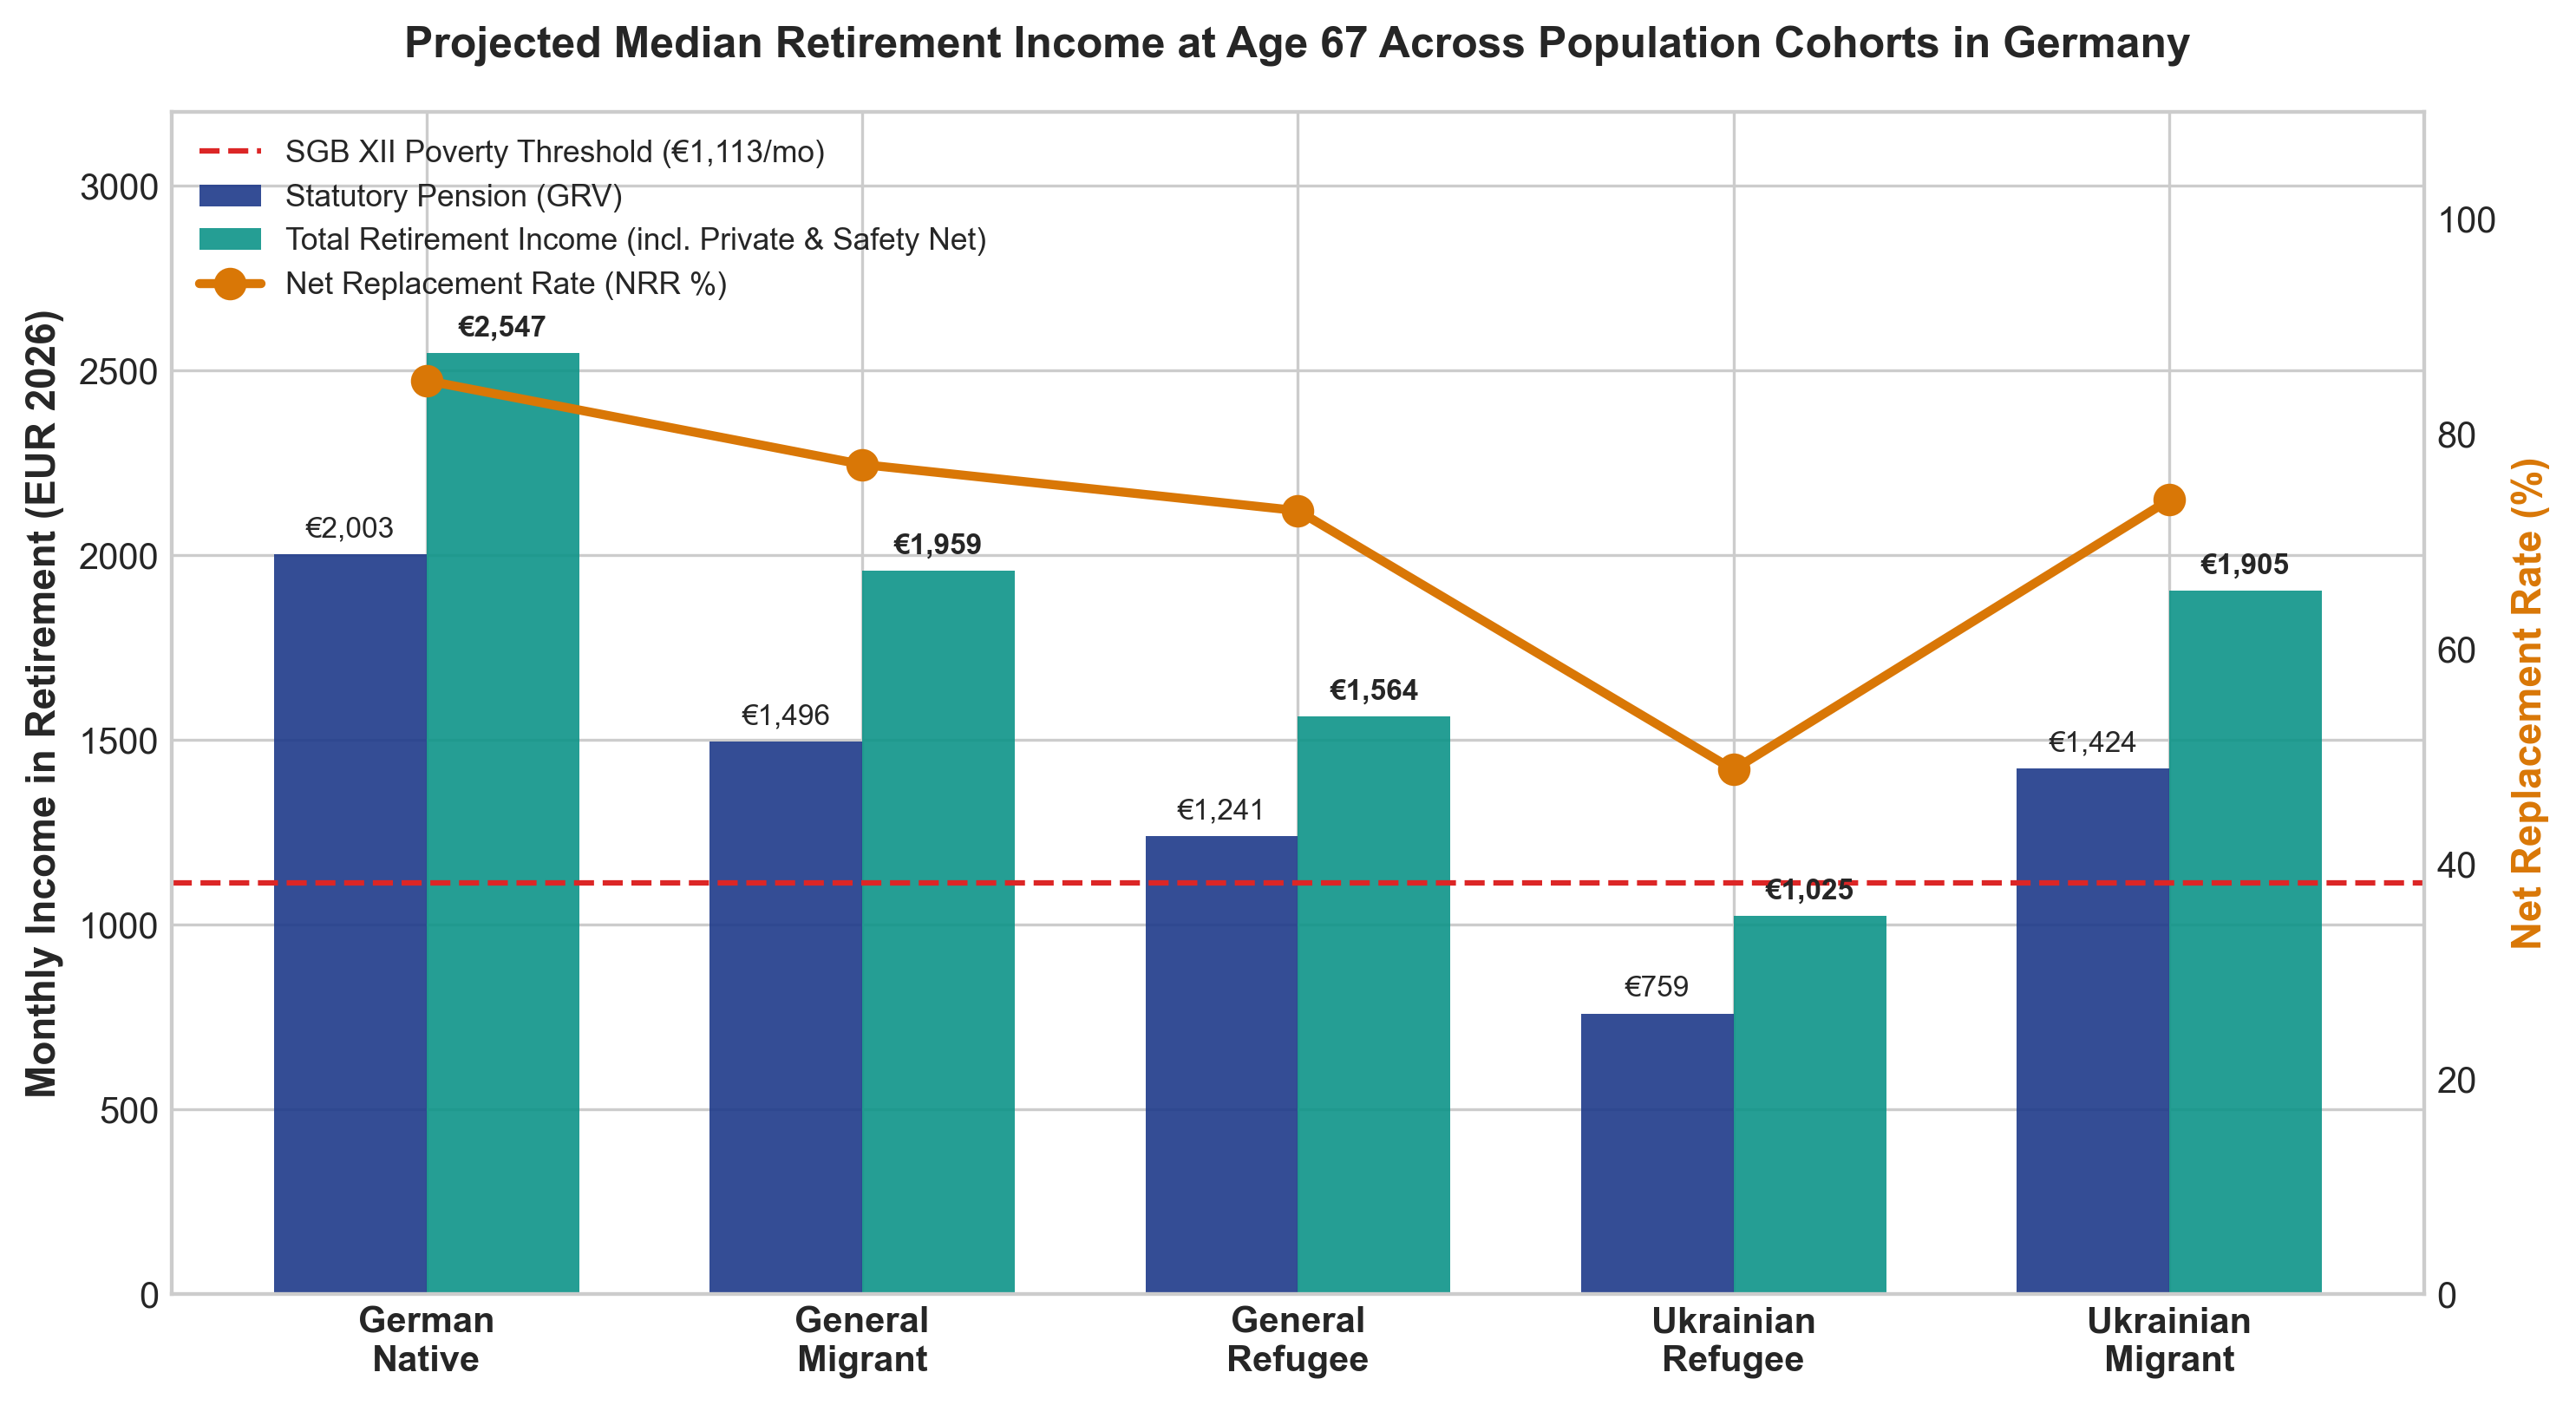
\includegraphics[width=0.95\columnwidth]{fig1_5way_retirement_income_and_nrr.png}
\caption{Projected median statutory pension (GRV) and total retirement income versus the illustrative SGB XII subsistence benchmark (\texteuro1,113/month).}
\label{fig:income_comp}
\end{figure}

\begin{figure}[htbp]
\centering
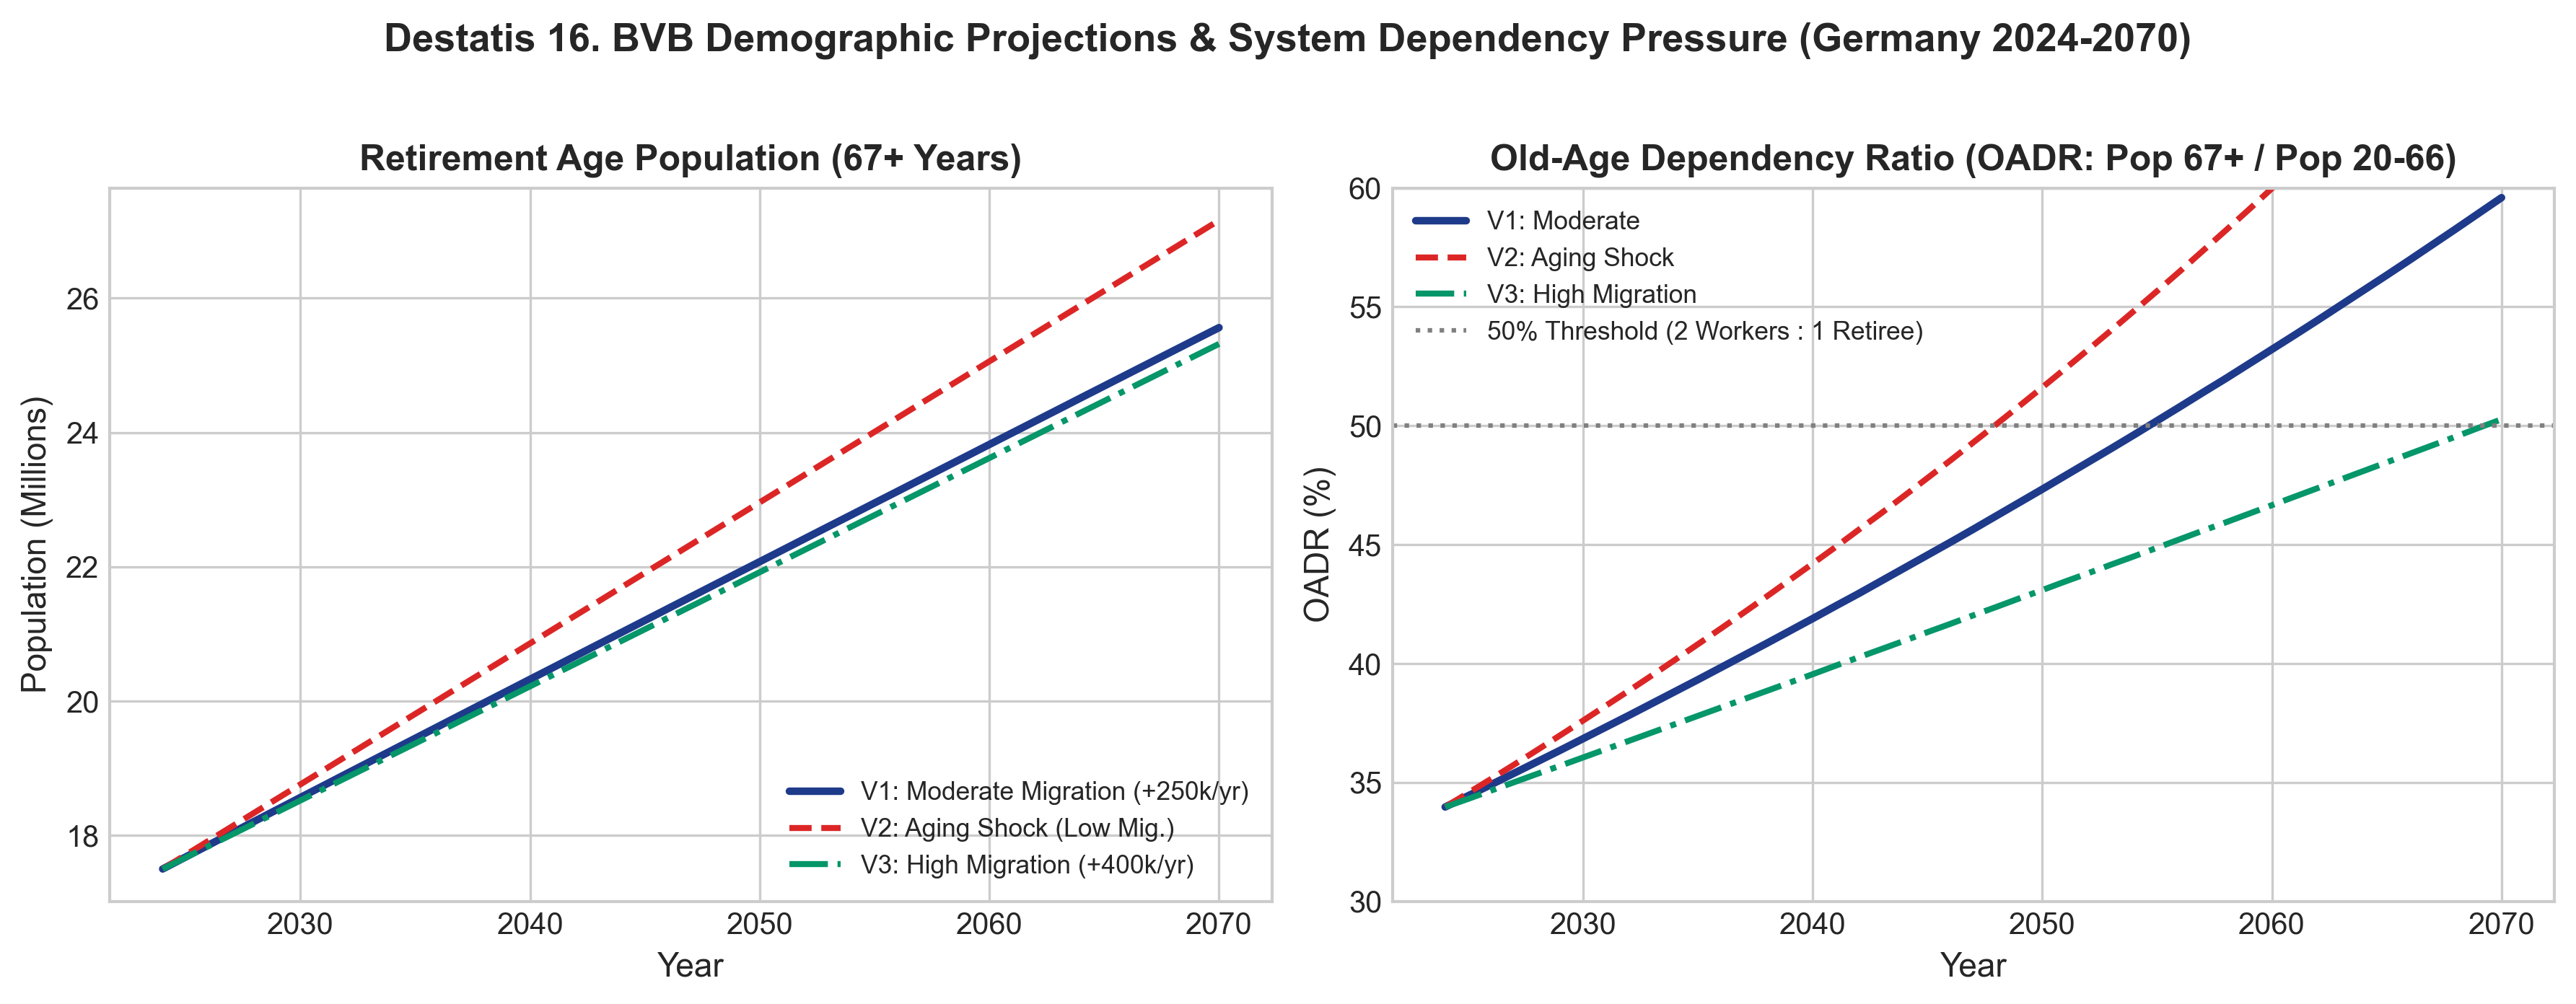
\includegraphics[width=0.95\columnwidth]{fig2_demographic_pressure_2070_oadr.png}
\caption{Destatis 16. BVB demographic projection scenarios and Old-Age Dependency Ratio (OADR) from 2024 to 2070.}
\label{fig:demog}
\end{figure}

\begin{figure}[htbp]
\centering
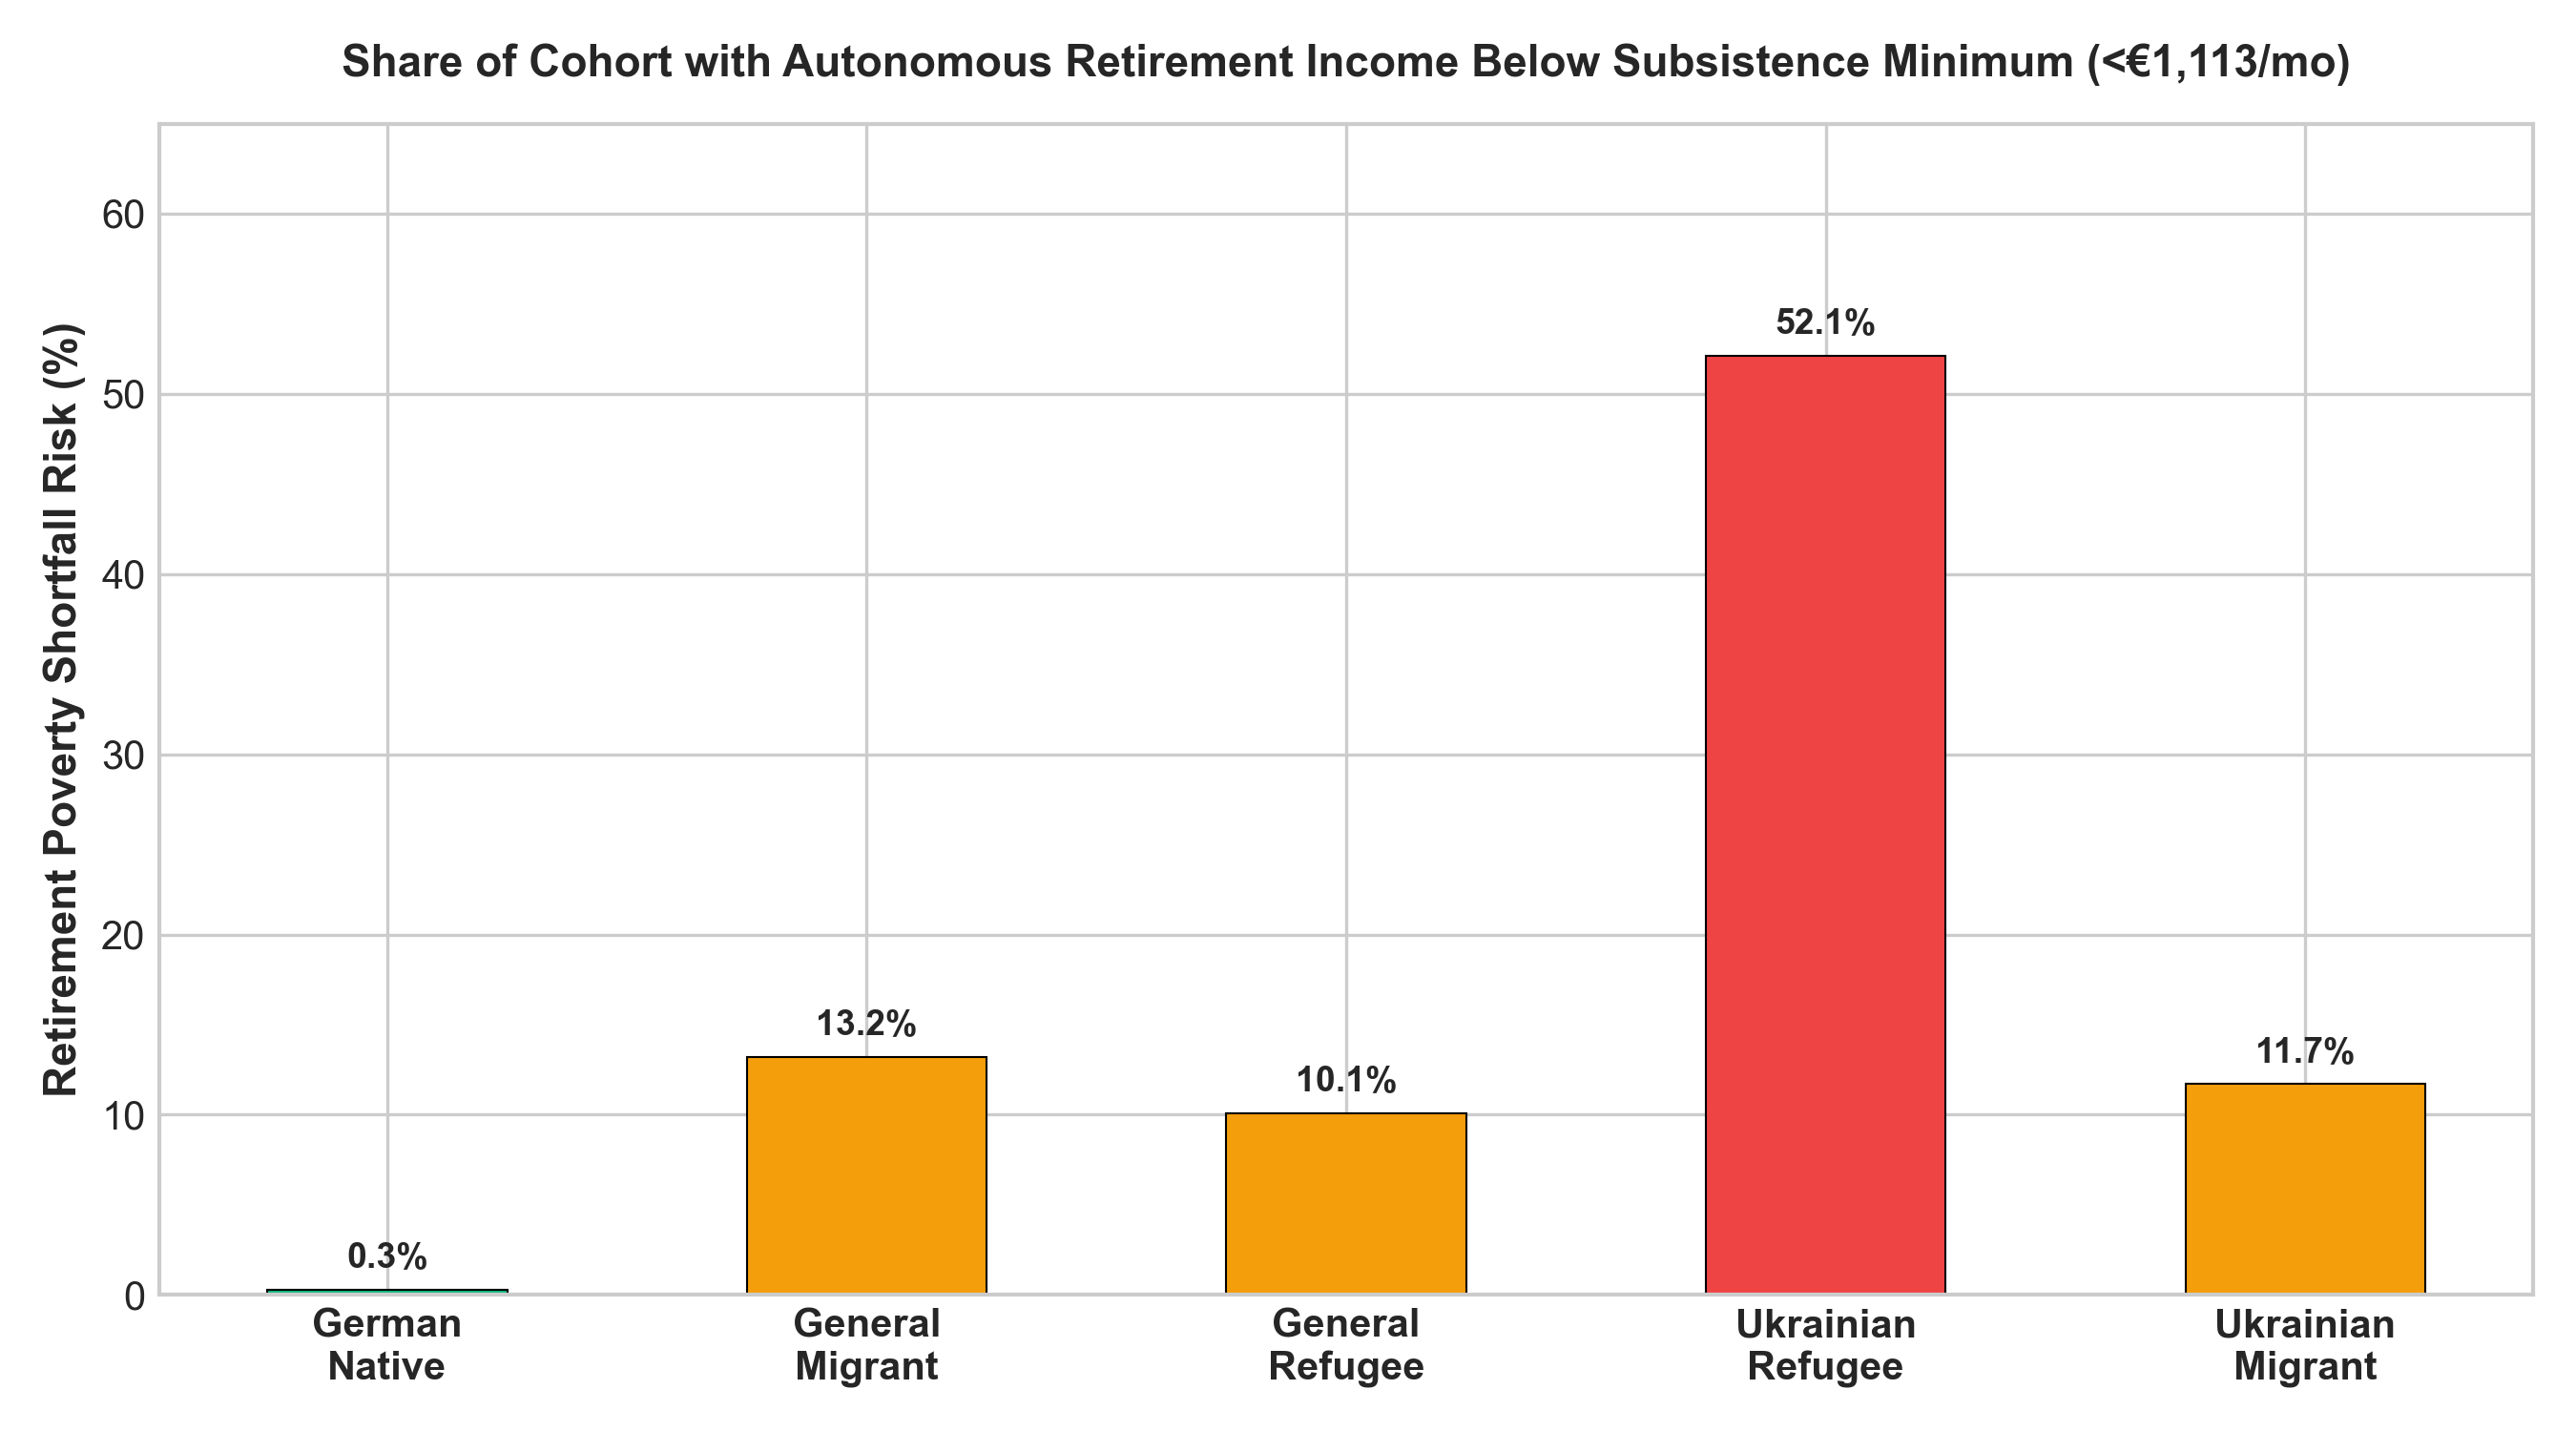
\includegraphics[width=0.95\columnwidth]{fig3_poverty_risk_and_savings_gap.png}
\caption{Illustrative subsistence gap ($<\text{\texteuro}1,113$/mo) and Required Additional Monthly Savings ($S^*$) across cohorts.}
\label{fig:poverty_gap}
\end{figure}

As shown in Table~\ref{tab:sim_results} and Fig.~\ref{fig:income_comp}, Ukrainian war refugees (2022+ arrivals) face a median statutory pension deficit (\texteuro804/mo), leaving 52.1\% (scenario sensitivity range: 44.6\%--58.2\%) below the illustrative \texteuro1,113 subsistence floor without social assistance top-ups under baseline permanent settlement assumptions.

\subsection{Required Additional Monthly Savings ($S^*$)}
We evaluate the individual capital accumulation effort needed to close the retirement shortfall via the Required Additional Monthly Savings $S^*$:
\begin{equation}
    S^* = \frac{\max\left(0, B_{\text{Target}} - [R_{\text{net}} + W_{\text{drawdown}}]\right) \cdot \ddot{a}_{\overline{K}|i}}{s_{\overline{N}|j}}
\end{equation}
where $B_{\text{Target}} = \max(\text{\texteuro}1,113, \min(\text{\texteuro}1,800, 0.60 \times w_{\text{net}}))$ represents the standard adequacy benchmark, $\ddot{a}_{\overline{K}|i} = (1 + i) \frac{1 - (1 + i)^{-12K}}{i}$ is the present value factor of an annuity-due over retirement horizon $K = 20$ years with monthly rate $i = r_{\text{post}}/12$, and $s_{\overline{N}|j} = \frac{(1 + j)^{12N} - 1}{j}$ is the ordinary future value accumulation factor over working horizon $N = 67 - \text{age}$ with monthly rate $j = r_{\text{pre}}/12$. Portfolio returns are expressed as annual real after-fee returns ($r_{\text{pre}} = 4.5\%, r_{\text{post}} = 2.0\%$). Timing assumes monthly savings contributed at the end of each working month and retirement withdrawals executed at the beginning of each retirement month.

\subsection{Sensitivity & Scenario Analysis}
To evaluate model robustness against key parameter uncertainties, Table~\ref{tab:sensitivity} reports sensitivity ranges across credential recognition rates, Ukrainian return migration, and asset returns.

\begin{table}[htbp]
\caption{Sensitivity Analysis for Post-2022 Ukrainian Refugee Cohort (Constant 2026 Euros)}
\centering
\begin{adjustbox}{width=\columnwidth}
\begin{tabular}{lcccccc}
\toprule
\textbf{Scenario Dimension} & \textbf{Variant} & \textbf{Stat. Pension} & \textbf{Priv. Drawdown} & \textbf{Total Income} & \textbf{Median NRR} & \textbf{Req. Savings $S^*$} \\
\midrule
\multirow{3}{*}{Foreign Credential Recognition} & 0\% (Status Quo) & \texteuro804 & \texteuro264 & \texteuro1,068 & 50.7\% & \texteuro180 / mo \\
 & 50\% Fast-Track & \texteuro1,095 & \texteuro325 & \texteuro1,420 & 61.2\% & \texteuro95 / mo \\
 & 100\% Full Match & \texteuro1,402 & \texteuro395 & \texteuro1,797 & 72.5\% & \texteuro35 / mo \\
\midrule
\multirow{3}{*}{Return Migration Trajectory} & 0\% (Full Settlement) & \texteuro804 & \texteuro264 & \texteuro1,068 & 50.7\% & \texteuro180 / mo \\
 & 30\% Partial Return & \texteuro852 & \texteuro280 & \texteuro1,132 & 52.8\% & \texteuro165 / mo \\
 & 60\% High Return & \texteuro918 & \texteuro305 & \texteuro1,223 & 55.4\% & \texteuro140 / mo \\
\midrule
\multirow{3}{*}{Real Equity Portfolio Return} & 2.0\% (Conservative) & \texteuro804 & \texteuro195 & \texteuro999 & 48.2\% & \texteuro220 / mo \\
 & 4.5\% (Baseline) & \texteuro804 & \texteuro264 & \texteuro1,068 & 50.7\% & \texteuro180 / mo \\
 & 6.0\% (Optimistic) & \texteuro804 & \texteuro340 & \texteuro1,144 & 54.1\% & \texteuro125 / mo \\
\bottomrule
\end{tabular}
\end{adjustbox}
\label{tab:sensitivity}
\end{table}

\section{Gender Dimension \& Methodological Boundaries}
Disaggregating by gender reveals structural divergence in absolute pensions consistent with differences in labor-market participation, part-time employment patterns, wage penalties ($-11.4\%$), and female longevity (Table~\ref{tab:gender_results}).

\begin{table}[htbp]
\caption{Gender-Disaggregated Median Outcomes at Age 67}
\centering
\begin{adjustbox}{width=\columnwidth}
\begin{tabular}{lcccc}
\toprule
\textbf{Cohort} & \textbf{Female Pension} & \textbf{Male Pension} & \textbf{Female NRR} & \textbf{Male NRR} \\
\midrule
German Native & \texteuro2,062 & \texteuro2,196 & 89.4\% & 85.7\% \\
General Migrant & \texteuro1,545 & \texteuro1,583 & 81.8\% & 77.5\% \\
General Refugee & \texteuro1,238 & \texteuro1,321 & 75.2\% & 74.5\% \\
Ukrainian Refugee & \texteuro775 & \texteuro902 & 50.0\% & 52.2\% \\
Ukrainian Migrant & \texteuro1,458 & \texteuro1,529 & 76.7\% & 75.7\% \\
\bottomrule
\end{tabular}
\end{adjustbox}
\label{tab:gender_results}
\end{table}

\section{Limitations \& Unmodeled Dimensions}
This microsimulation framework relies on several explicit modeling boundaries:
\begin{enumerate}
    \item \textbf{Causal Identification}: Mincerian wage and IHS wealth regressions reflect conditional statistical associations rather than quasi-experimental causal treatment effects.
    \item \textbf{Deterministic Retirement Horizon}: The baseline savings calculation assumes a deterministic 20-year retirement horizon ($K=20$, ages 67--87) and does not model individual mortality hazards or morbidity-driven early exits.
    \item \textbf{Intra-Household Wealth Pooling}: The model operates primarily at the individual level; married couples often pool wealth and living expenses, buffering single-adult subsistence risks.
    \item \textbf{Derived Rights \& Survivor Pensions}: Derived entitlements such as statutory widow/widower pensions (\S~46 SGB VI) and pension rights adjustment upon divorce (\textit{Versorgungsausgleich}) are not explicitly simulated.
    \item \textbf{Foreign Pension Portability}: Reported retirement income represents German retirement entitlements and excludes potentially portable foreign pension rights accrued prior to migration due to data limitations.
    \item \textbf{Future Legislative Uncertainty}: The model applies currently legislated institutional rules and statutory indexation mechanisms but does not anticipate future discretionary major legislative structural reforms.
\end{enumerate}

\section{Policy Recommendations}
\begin{enumerate}
    \item \textbf{Fast-Track Credential Recognition}: Accelerated qualification homologation under the \textit{Berufsqualifikationsfeststellungsgesetz} could substantially reduce the wage disadvantage associated with qualification mismatch. Under the modeled full-recognition counterfactual scenario, 78.4\% of vulnerable refugee workers who would otherwise experience qualification mismatch achieve autonomous retirement adequacy above \texteuro1,113/month.
    \item \textbf{Capital-Funded Pension Wrappers (\textit{Altersvorsorgedepot})}: A potential policy reform could introduce individual tax-sheltered investment accounts to enable late-entry migrants to close the $S^*$ savings gap through equity market compounding.
    \item \textbf{Adjustment of SGB XII Disregard Rules (\S~82a)}: Adjusting the statutory income disregard could strengthen the financial incentive to accumulate contributory pension rights, particularly for low-income workers with qualifying insurance histories.
\end{enumerate}

\section{Conclusion \& Open Reproducibility}
This study develops a calibrated dynamic microsimulation framework assessing retirement adequacy under multi-cohort migration dynamics through 2070. All code, synthetic datasets, and the interactive multilingual dashboard are openly available for scientific replication.

\section*{Acknowledgment}
This research platform and simulation pipeline were developed under the scientific direction of Cristhian David Caceres Mateus. Computational modeling and econometric pipelines were engineered in Antigravity (Google DeepMind).

\bibliographystyle{IEEEtran}
\bibliography{references}

\end{document}
